\documentclass[tikz,border=2pt]{standalone}
\usepackage{amsmath,amssymb}
\usepackage{pgfplots}
\pgfplotsset{compat=1.18}
\usetikzlibrary{arrows.meta}
\begin{document}
% LER as an area ratio: for X ~ Exp(0.01) the area under bar F_X(t) = e^{-0.01t} is E[X] = 100;
% the part on [0,d], d = 100, is E[min(X,d)] = 100(1-e^{-1}) ~ 63.2, the rest pi_X(d) = 100e^{-1} ~ 36.8.
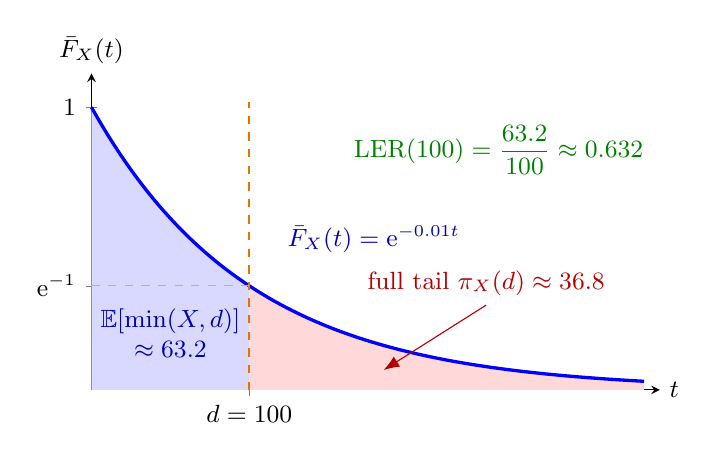
\begin{tikzpicture}[font=\small, >={Latex[length=2mm]}]
  \begin{axis}[
    axis lines=left, xmin=0, xmax=360, ymin=0, ymax=1.12,
    xtick={100}, xticklabels={$d=100$}, ytick={0.368,1}, yticklabels={$\mathrm{e}^{-1}$,$1$},
    xlabel={$t$}, ylabel={$\bar F_X(t)$},
    xlabel style={at={(axis description cs:1,0)}, anchor=west},
    ylabel style={rotate=-90, at={(axis description cs:0,1)}, anchor=south},
    samples=100, width=8.8cm, height=5.6cm, clip=false]
    \addplot[fill=blue!15, draw=none, domain=0:100] {exp(-0.01*x)} \closedcycle;
    \addplot[fill=red!15, draw=none, domain=100:350] {exp(-0.01*x)} \closedcycle;
    \addplot[blue, very thick, domain=0:350] {exp(-0.01*x)};
    \draw[orange!90!black, thick, dashed] (axis cs:100,0) -- (axis cs:100,1.02);
    \draw[gray!60, thin, dashed] (axis cs:0,0.368) -- (axis cs:100,0.368);
    \node[blue!70!black, align=center] at (axis cs:50,0.2) {$\mathbb{E}[\min(X,d)]$\\$\approx63.2$};
    \draw[red!70!black, ->] (axis cs:250,0.3) -- (axis cs:185,0.07);
    \node[red!70!black, anchor=south] at (axis cs:250,0.3) {full tail $\pi_X(d)\approx36.8$};
    \node[blue!70!black, anchor=south west] at (axis cs:118,0.45) {$\bar F_X(t)=\mathrm{e}^{-0.01t}$};
    \node[green!50!black, anchor=west] at (axis cs:160,0.85) {$\operatorname{LER}(100)=\dfrac{63.2}{100}\approx0.632$};
  \end{axis}
\end{tikzpicture}
\end{document}
